\documentclass[xcolor=pst,dvips,12pt,english,french]{beamer}
\usepackage[backend=biber,style=numeric,firstinits=true, isbn=false, url=false, doi=false, eprint=false]{biblatex}

\bibliography{../biblio.bib}
\usepackage{graphicx}
\usepackage{babel}
\usepackage[utf8]{inputenc}
\usepackage{lmodern}
\usepackage{beamerthemeshadow}
\usepackage[skip=2pt,font=scriptsize,labelformat=empty]{caption} % Required for specifying captions to tables and figures
%\usepackage{pstricks}

\title{Apprendre par joint-attention ?}
\author{Fournier Pierre}

\addtobeamertemplate{navigation symbols}{}{%
	\usebeamerfont{footline}%
	\usebeamercolor[fg]{footline}%
	\hspace{1em}%
	\insertframenumber/\inserttotalframenumber
}


\begin{document}
	\frame{\titlepage} 
	
	%\frame{\frametitle{Table of contents}\tableofcontents} 
	
	\begin{frame}{Objectif}
		\begin{block}{}
			Etant donné un robot \textbf{autonome} en présence d'êtres humains, comment ces derniers peuvent susciter et guider l'apprentissage de \textbf{nouveaux comportements} par leur \textbf{interaction naturelle} (= sans intervention informatique) avec le robot ?
		\end{block}
		\begin{exampleblock}{}
			\textbf{Applications} : 
			\begin{itemize}
				\item Personnalisation d'un robot de compagnie 
				\item Spécialisation d'un robot industriel 
			\end{itemize}
		\end{exampleblock}
	\end{frame}
	
	\begin{frame}{Cadre et approche choisis}
		\begin{block}{}
			\textbf{But} : orienter l'exploration autonome du robot vers une version d'une tâche 
		\end{block}
		\begin{columns}
			\begin{column}{0.4\textwidth}
				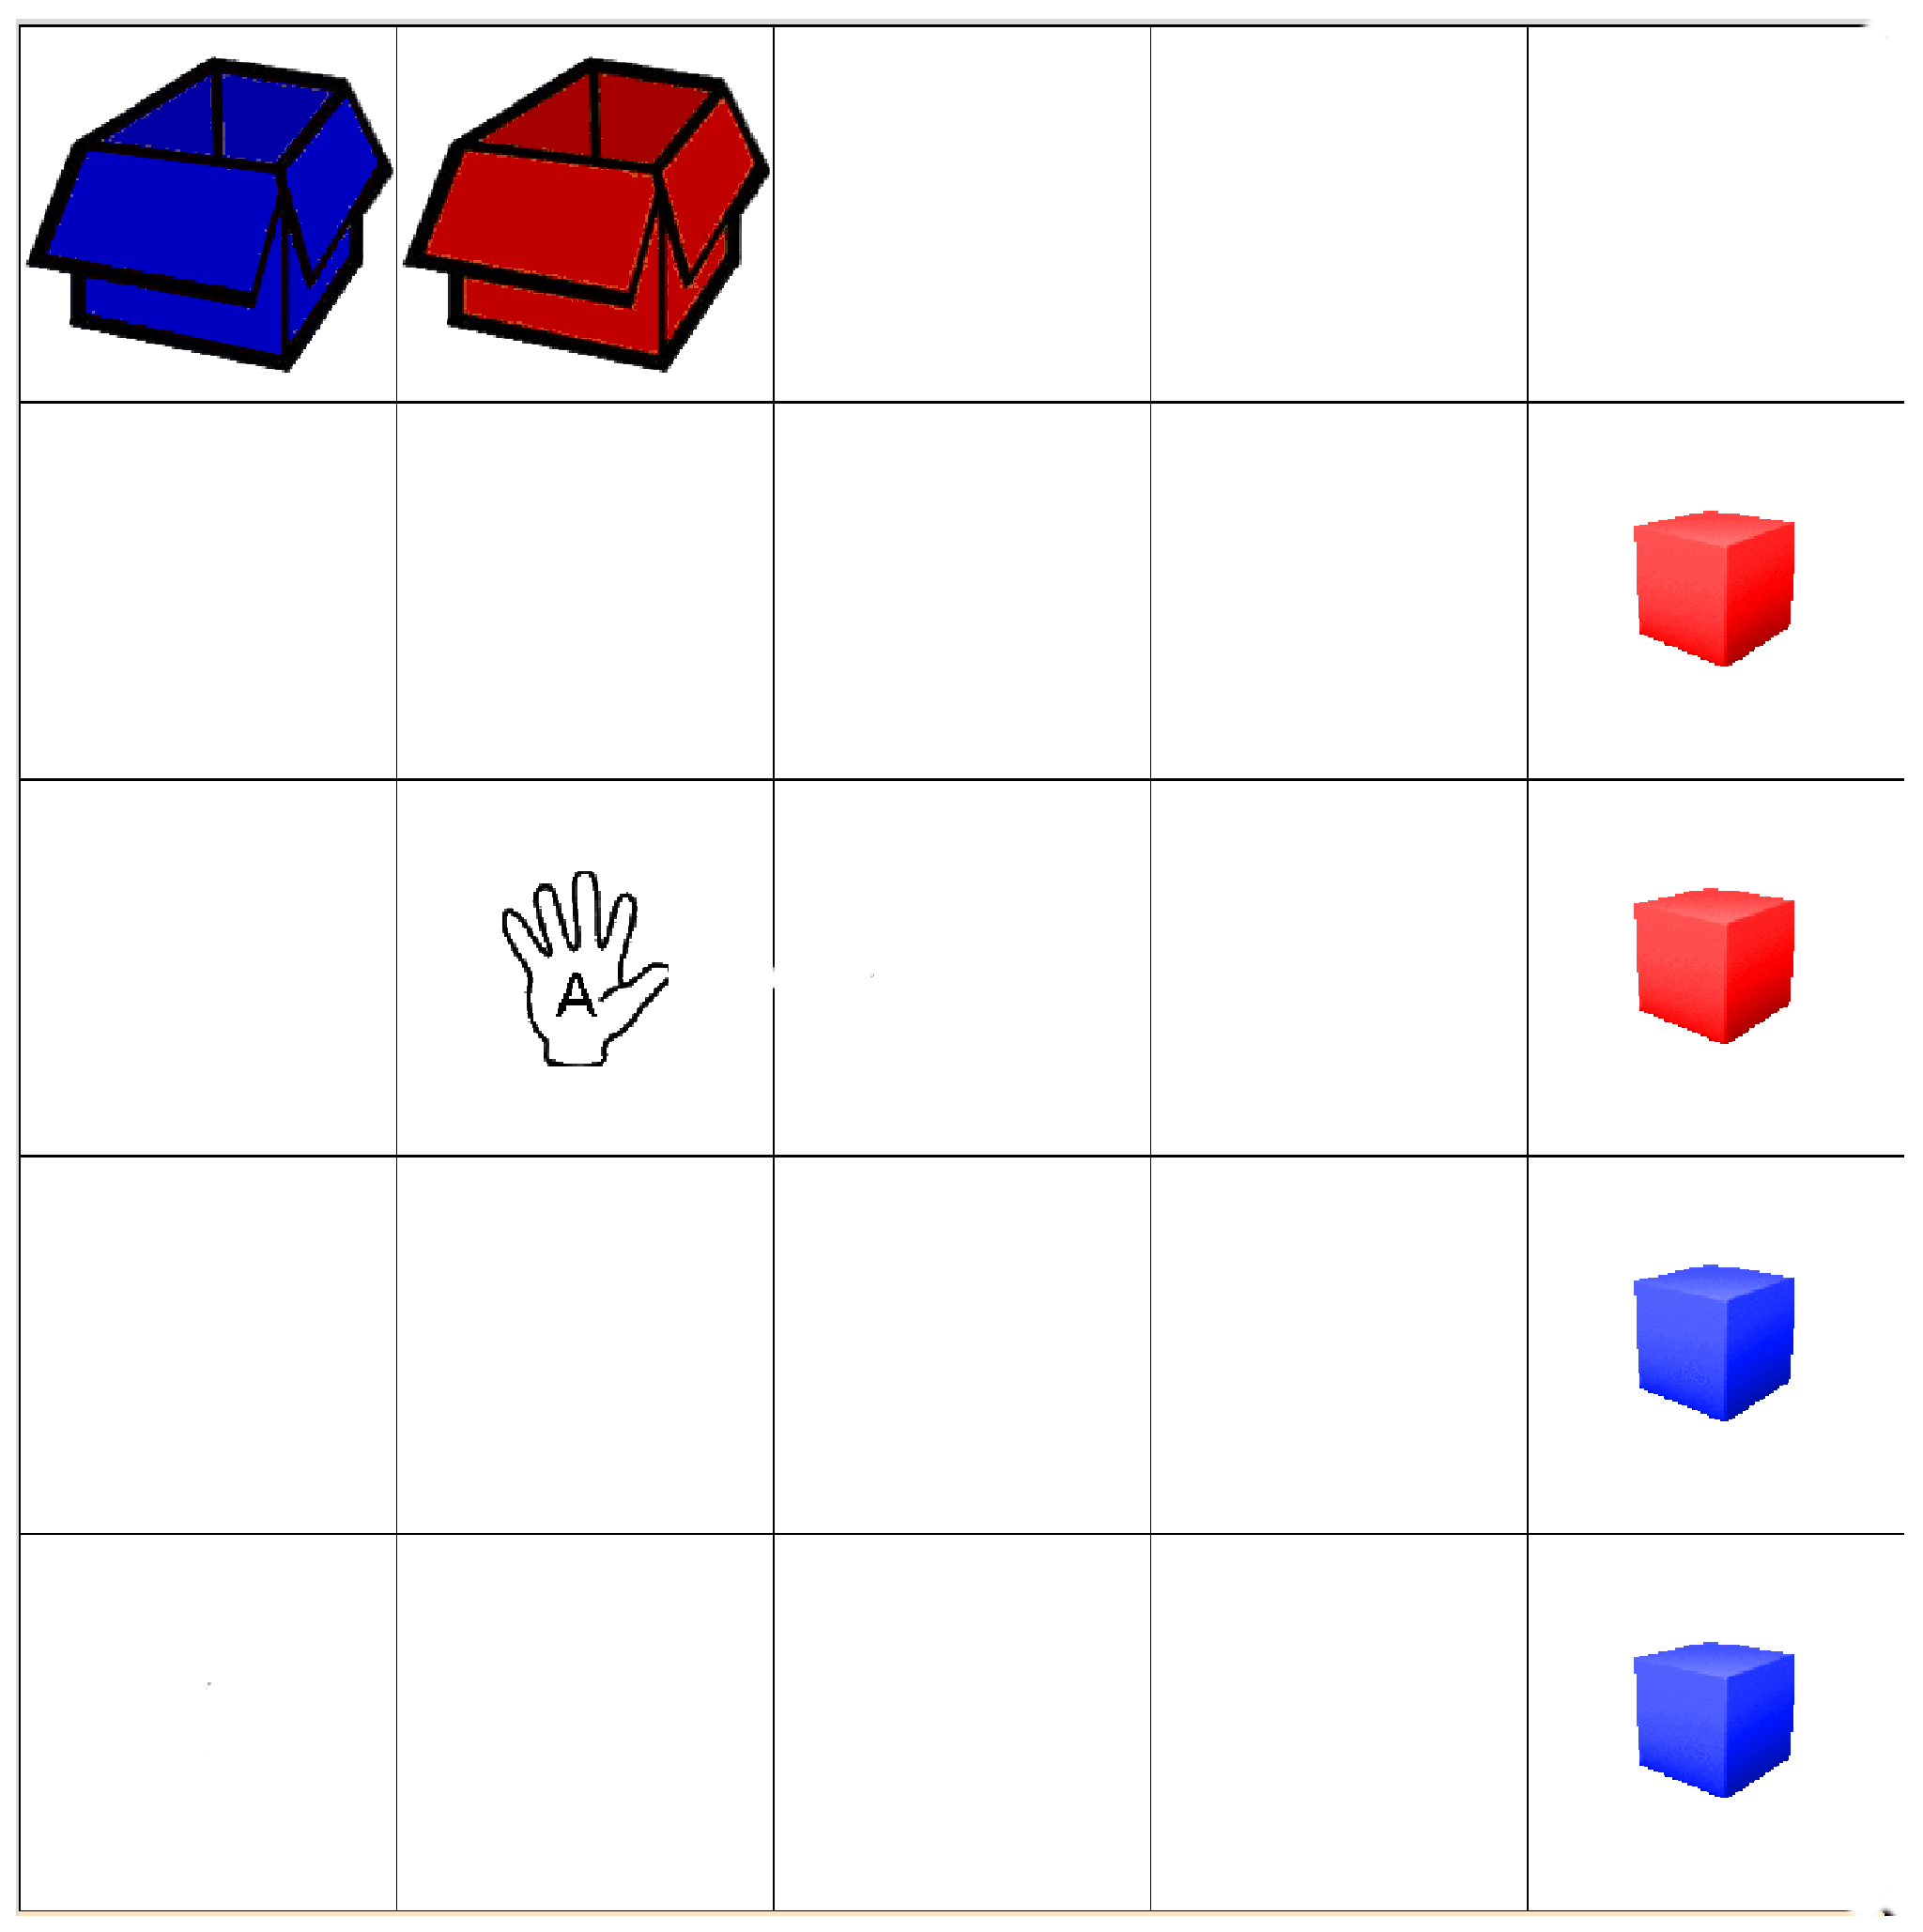
\includegraphics[width=\textwidth]{images/playroom1.eps}
			\end{column}
			\begin{column}{0.45\textwidth}
				\begin{block}{}
					\textbf{Sous-problèmes :}
					\begin{itemize}
						\item Implémenter un agent autonome explorant un environnement 
						\item Diriger l'exploration par une interaction homme robot naturelle
					\end{itemize}
				\end{block}
			\end{column}
		\end{columns}
	\end{frame}
	
	\begin{frame}{Exploration autonome}
		
		\begin{block}{}
			\textbf{Objectif} : découverte de séquences d'interactions pertinentes avec son environnement.
		\end{block}
		\begin{exampleblock}{}
			\textbf{Solution classique} : reinforcement learning. Des états de l'environnements sont "récompensants" et l'agent cherche un comportement décisionnel maximisant la récompense espérée.
		\end{exampleblock}
		\begin{columns}
			\begin{column}{0.4\textwidth}
				\centering
				\includegraphics[width=\textwidth, trim={0 0 1cm 0, clip}]{images/RL1.eps}
			\end{column}
			\begin{column}{0.5\textwidth}
				\begin{alertblock}{}
					\textbf{Problème} : peu de récompenses "naturelles" dans l'environnement, et les définir a priori réduit l'adaptabilité du robot.
				\end{alertblock}
			\end{column}
		\end{columns}
		\vfill
		\tiny
		\fullcite{sutton1998}

	\end{frame}
	
	\begin{frame}{Motivation intrinsèque}
		\begin{block}{}
			\textbf{Solution} : le robot s'attribue lui-même des récompenses selon un/des objectif(s) indépendant(s) de toute tâche. 
		\end{block}
		\begin{exampleblock}{}
			\textbf{Exemples} : 
			\begin{itemize}
				\item Découverte autonome de buts
				\item \textbf{Curiosité artificielle} : maximisation de la compétence, de la prédictibilité, etc.
				\item Recours à un méta-modèle pour l'évaluation du modèle et la définition de l'objectif générique
			\end{itemize}
		\end{exampleblock} 
		\vfill
		\tiny
		\fullcite{chentanez2004}
		\\
		\fullcite{oudeyer2007}
	\end{frame}
	
	\begin{frame}{Mise en \oe{}uvre}
		\begin{block}{}
			\textbf{Un modèle prédictif de l'environnement avec} : 
			\begin{itemize}
				\item Une mesure de l'incertitude 
				\item Une mesure de la nouveauté 
			\end{itemize}
		\end{block}
		\begin{columns}
			\begin{column}{0.4\textwidth}
				\centering
				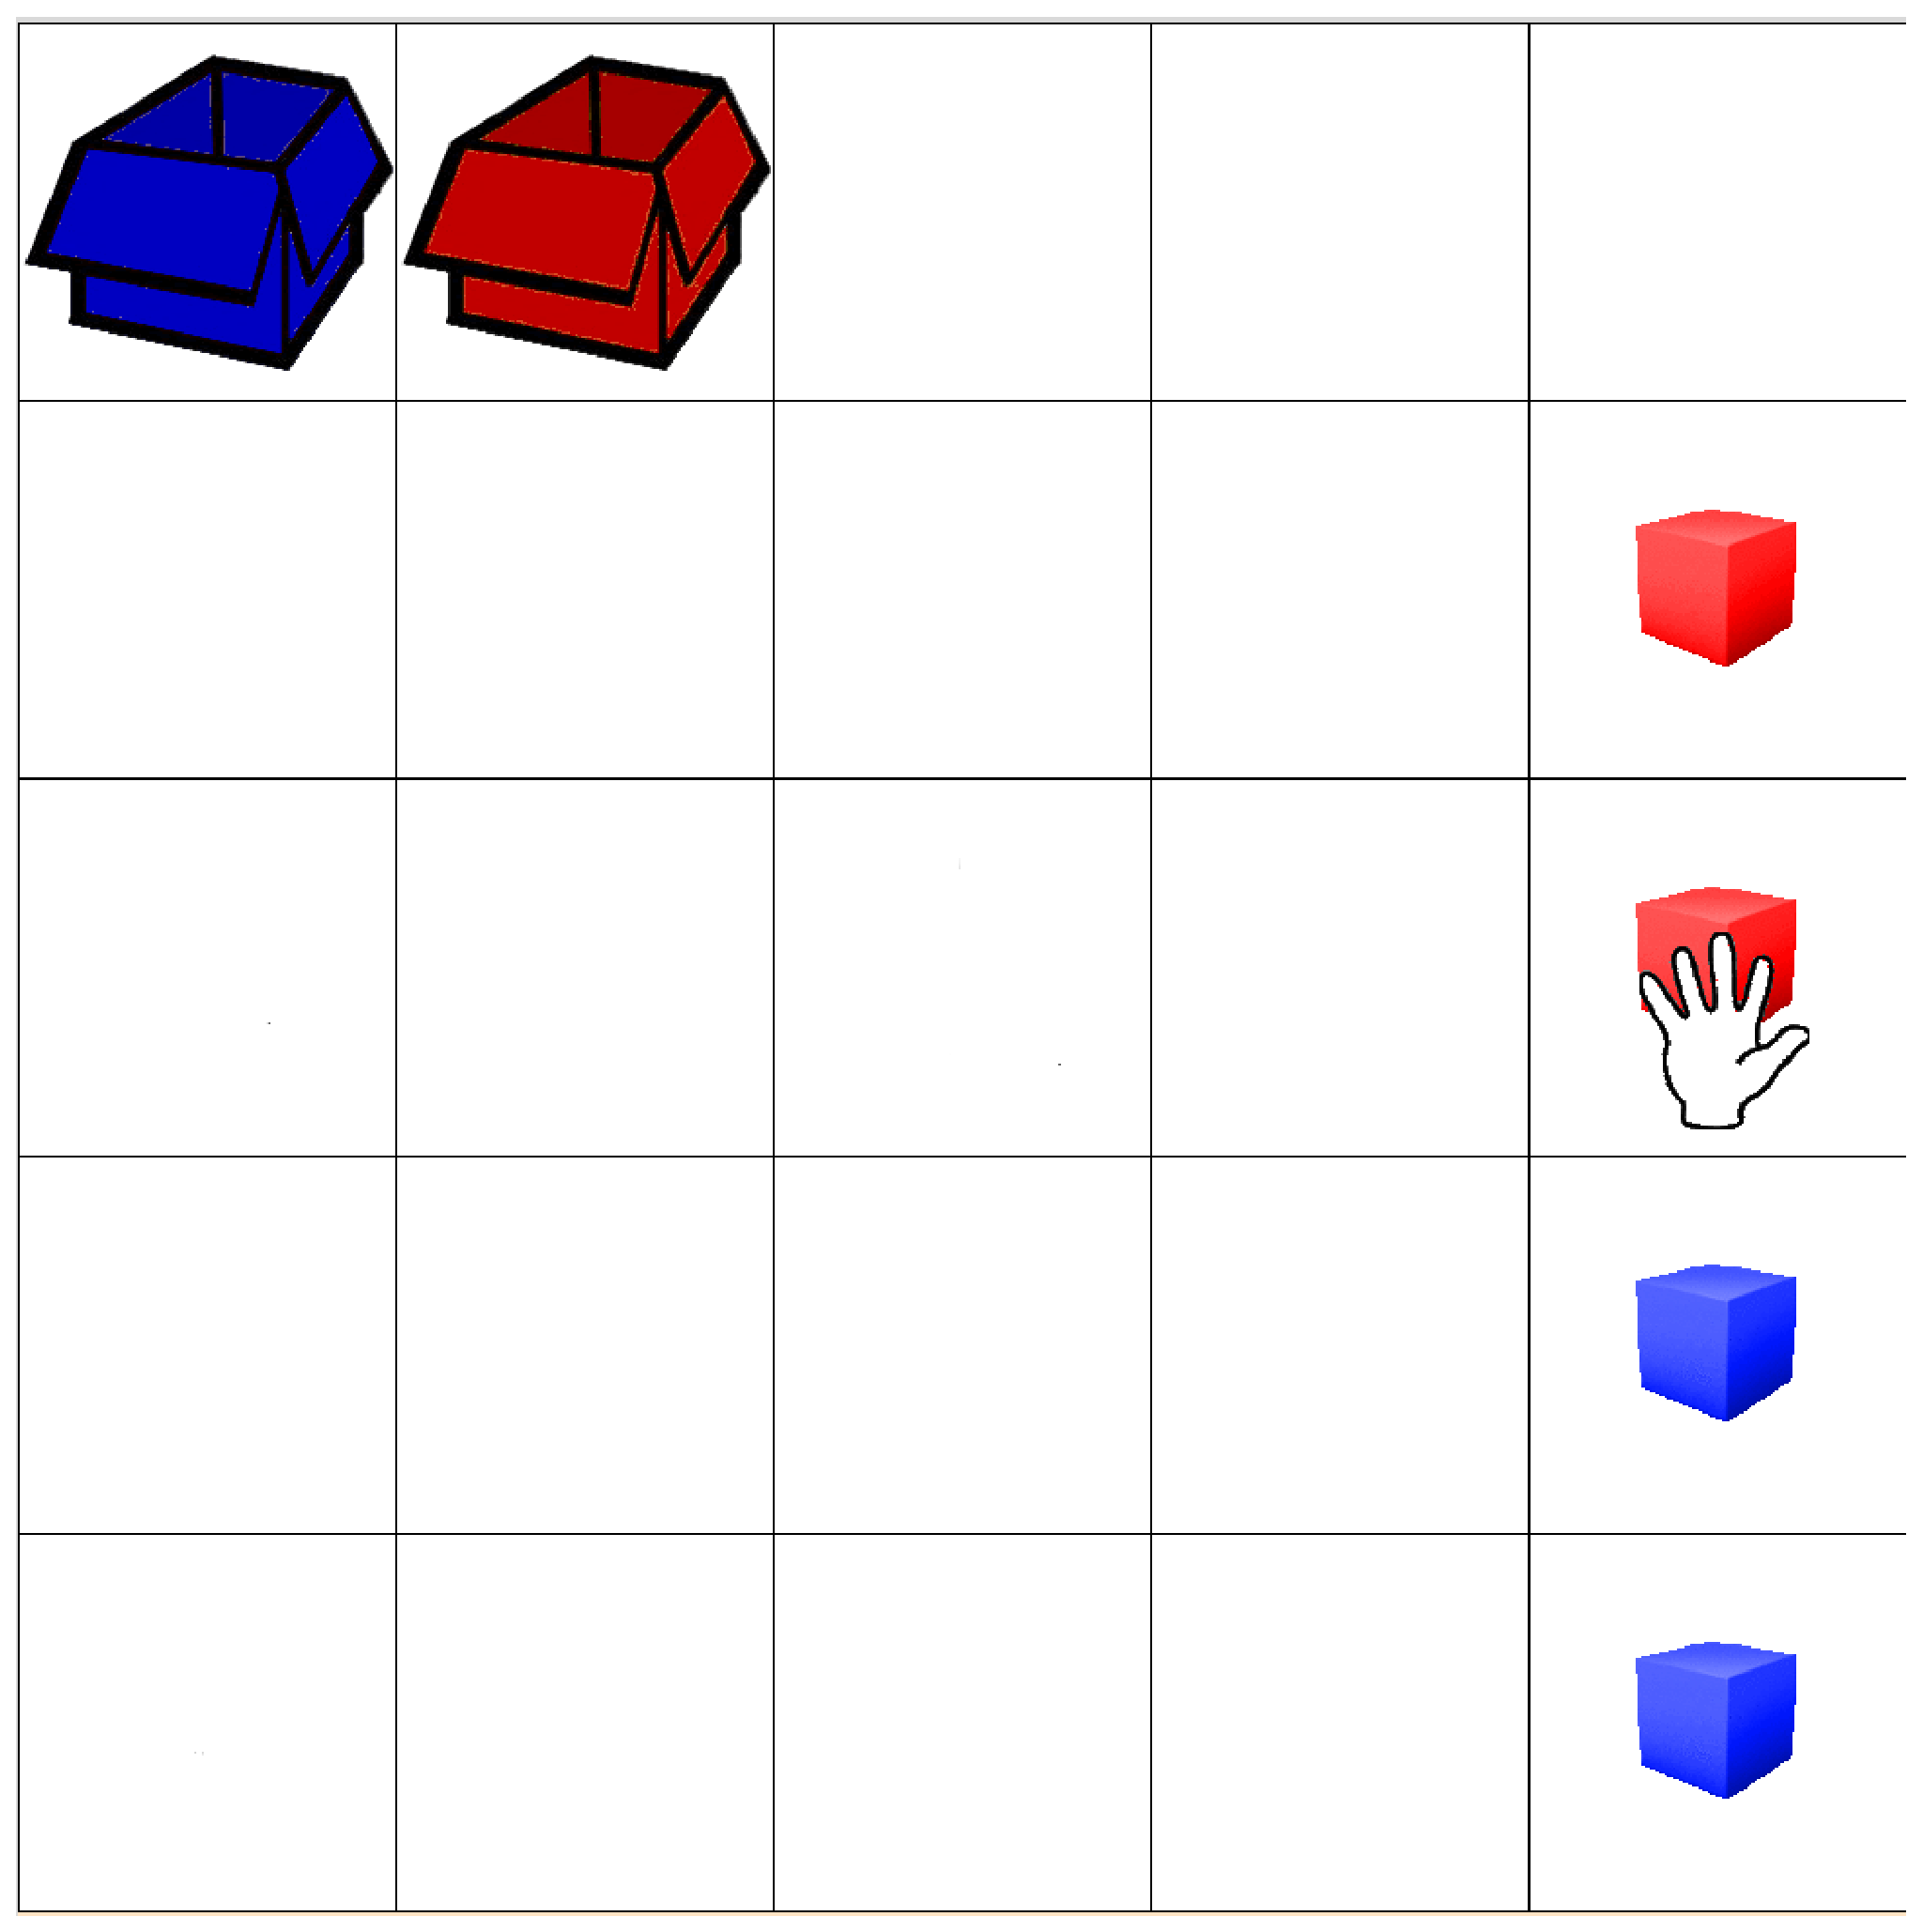
\includegraphics[width=\textwidth, trim={0 0 1cm 0, clip}]{images/playroom3.eps}
			\end{column}
			\begin{column}{0.5\textwidth}
				\begin{alertblock}{}
					\begin{itemize}
						\item Déplacements discrets dans la grille
						\item Actions avec probabilité de réussite selon l'état
						\item Cadre RL classique avec reward shaping pour inclure les deux mesures de motivation intrinsèque
					\end{itemize}
				\end{alertblock}
			\end{column}
		\end{columns}
	\end{frame}
	
	\begin{frame}{Guider l'exploration par l'interaction}
		\begin{block}{}
			\textbf{Problème} : comment insérer l'interaction dans le cadre de l'exploration autonome par curiosité artificielle ?
		\end{block}
		\begin{exampleblock}{}
			\textbf{Observation} : une interaction positive est valorisée par l'enfant, indépendamment de son but, et une interaction négative est perçue comme désagréable\\
			\textbf{Exemple} : attrait pour les jeux sociaux (peek-a-boo...), ré-engagement de l'interaction, still face experiments
		\end{exampleblock}
		\begin{alertblock}{}
			\textbf{Problème} : comment exploiter ce constat ? Qu'est-ce qui différencie une interaction positive d'une interaction négative ?
		\end{alertblock}
		\vfill
		\tiny
		\fullcite{parrott1989}
		\\
		\fullcite{adamson2003}
	\end{frame}
	
	\begin{frame}{Joint attention}
		\begin{block}{}
			\begin{itemize}
				\item Attention detection (gaze following) 
				\item Attention manipulation (pointing)
				\item Social coordination (rythme)
				\item Intentional stance (goal directed behaviours)
			\end{itemize}
		\end{block}
		\begin{exampleblock}{}
			\textbf{Principe} : faire de la joint-attention une seconde source de renforcement primaire, au même titre que satisfaire la curiosité, et l'utiliser pour transférer l'intention du tuteur à l'agent.
		\end{exampleblock}	
		\vfill
		\tiny
		\fullcite{kaplan2006challenges}
	\end{frame}
	
	\begin{frame}{Questions de modélisation}
		\begin{block}{}
			Quelle est la source du renforcement ? Comment éviter de "ne faire qu'interagir" ?
		\end{block}
		\begin{columns}
			\begin{column}{0.4\textwidth}
				\centering
				\includegraphics[width=\textwidth, trim={0 0 1cm 0, clip}]{images/playroom2.eps}
			\end{column}
			\begin{column}{0.5\textwidth}
				\begin{alertblock}{}
					\begin{itemize}
						\item Nécessité des 4 points de la joint attention ?
						\item Attention jointe innée ou acquise ?
						\item Possibilité pour le tuteur d'attribuer une récompense externe pure à l'agent ?
					\end{itemize}
				\end{alertblock}
			\end{column}
		\end{columns}
	\end{frame}
	
	\begin{frame}{Related work}
		\begin{block}{}
			\begin{itemize}
				\item \small
				\citetitle{knox2009}, \citeauthor{knox2009}.\\
				\textbf{Différences} : cadre d'apprentissage fixé, signaux humains pré-interprétés.
				\item \small
				\citetitle{najar}, \citeauthor{najar}.\\
				\textbf{Différences} : renforcements secondaires fournis par l'environnement, association one--to--one geste/instruction
				\item \small
				\citetitle{grand2014}, \citeauthor{grand2014}.\\
				\textbf{Différences} : synchronie temporelle uniquement, requiert un utilisateur très engagé.
			\end{itemize}
		\end{block}
	\end{frame}
	

	
	
	

	
%	\begin{frame}{La robotique développementale}
%		\begin{block}{Un robot peut-il apprendre comme un enfant ?}
%			 Privilégier l'apprentissage de compétences bas niveau et mettre en place une architecture structurée permettant la progression autonome.
%		\end{block}
%		\begin{columns}
%			\begin{column}{0.45\textwidth}
%				\begin{exampleblock}{Contraintes}
%					\begin{itemize}
%						\item \emph{Lifelong learning}
%						\item \emph{task-independent architecture}
%						\item Complexité croissante des compétences
%					\end{itemize}
%				\end{exampleblock}
%			\end{column}
%			\begin{column}{0.45\textwidth}
%				\begin{exampleblock}{Inspiration}
%					Psychologie développementale, neurosciences, linguistique, biologie évolutionnaire...
%				\end{exampleblock}
%			\end{column}
%		\end{columns}
%	\end{frame}
%	
%	\begin{frame}{Interagir avec un environnement}
%		\begin{block}{Embodied, situated robots}
%			La cognition émerge chez un organisme par l'interaction avec son environnement, dépendante des capacités sensorimotrices de l'organisme dans cet environnement.
%		\end{block}
%		\begin{columns}
%			\begin{column}{0.55\textwidth}
%				\begin{exampleblock}{Autonomous object discovery}
%					Interaction avec des objets : 
%					\begin{itemize}
%						\item Identification
%						\item Apprentissage d'affordances
%						\item Séquences d'actions
%					\end{itemize}
%				\end{exampleblock}
%			\end{column}
%			\begin{column}{0.35\textwidth}
%				\vspace{0.5cm}
%				\centering
%				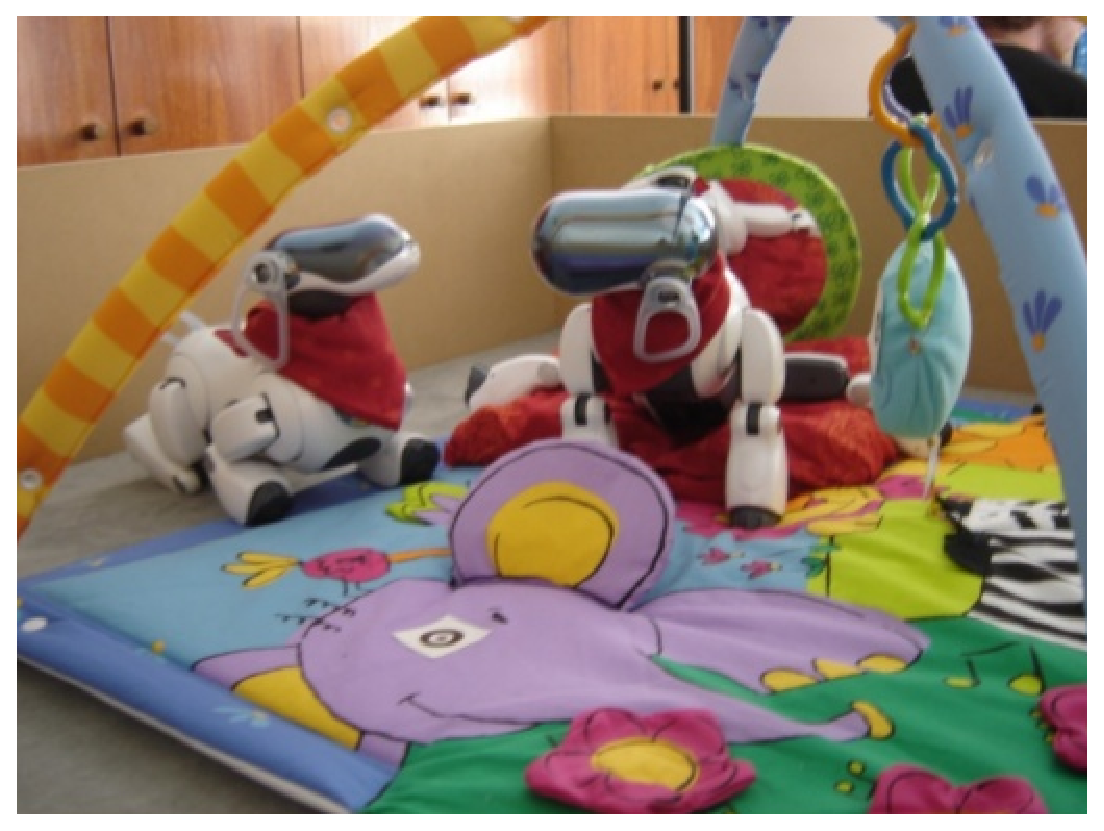
\includegraphics[width=\textwidth]{images/playground.eps}
%				\captionof{figure}{The playground experiment}
%			\end{column}
%		\end{columns}
%	\end{frame}
%	
%	\subsection{Intrinsically motivated reinforcement learning}
%	
%	
%	
%	\section{Positionnement de la thèse}
%
%	\begin{frame}{Positionnement de la thèse}
%		\begin{block}{Guidage de l'exploration}
%			Au sein d'une tâche de découverte autonome d'un environnement, comment guider et accélérer l'exploration du robot par une interaction avec un tuteur humain ?
%		\end{block}
%		\begin{exampleblock}{Applications hors apprentissage développemental}
%			Personnalisation / amélioration des compétences d'un robot de manière naturelle et sans recourir à la programmation.
%			 \\ 
%			$\to\,$ Jeu avec un robot de compagnie par exemple.
%		\end{exampleblock}
%	\end{frame}
%	
%	\subsection{Interactive reinforcement learning}
%	
%	\begin{frame}{Interactive reinforcement learning}
%		\begin{block}{Principe}
%			La récompense provient partiellement d'une interaction en temps réel avec un tuteur (démonstration, guidage,...)
%		\end{block}
%		\begin{exampleblock}{Labeled to unlabeled guidance}
%			L'interprétation de l'interaction n'a pas de raison d'être connue du robot :
%			\begin{itemize}
%				\item Apprentissage de la tâche 
%				\item Apprentissage du sens de l'interaction
%			\end{itemize}
%		\end{exampleblock}
%	\end{frame}
%	
%	\begin{frame}{Réflexion sur l'interaction}
%		\begin{block}{Constat chez les enfants}
%			L'interaction elle-même semble être valorisée indépendamment de son objet : aide spontanée, reproduction d'un jeu une fois appris, etc.
%		\end{block}
%		\begin{exampleblock}{But des expériences futures}
%			En attribuant au sein du mécanisme de motivation intrinsèque une valeur positive à la synchronie entre agent et tuteur, est-il possible de guider l'exploration autonome dans la direction manifestée par les actions du tuteur ? 
%		\end{exampleblock}
%	\end{frame}
%	
%	\subsection{Cadre actuel}
%	
%	\begin{frame}{Cadre de travail actuel}
%		\begin{columns}
%			\begin{column}{0.55\textwidth}
%				\includegraphics[width=\textwidth]{images/playroom.eps}
%			\end{column}
%			\begin{column}{0.45\textwidth}
%				\begin{block}{Synchrony-based guidance ?}
%					\begin{itemize}
%						\item Espace discrétisé
%						\item Agent \& Tuteur : regard, intention, action
%						\item Des boîtes et des blocs à ranger
%						\item Un interrupteur nécessaire pour distinguer les couleurs
%					\end{itemize}
%				\end{block}
%			\end{column}
%		\end{columns}
%	\end{frame}

\end{document}